%%%%%%%%%%%%%%%%%%%%%%%%%%%%%%%%%%%%%%%% IMPORTS %%%%%%%%%%%%%%%%%%%%%%%%%%%%%%%%%%%%%%%%
\documentclass[11pt,a4paper]{article}

%%%%%%%%%%%%%%% Formatting %%%%%%%%%%%%%%% 
\usepackage[english]{babel}
\usepackage[utf8]{inputenc}
\usepackage{geometry} % Margins
\usepackage{sectsty} % Custom Sections

%%%%%%%%%%%%%%% Font %%%%%%%%%%%%%%% 
\usepackage{Archivo}
\usepackage[T1]{fontenc}

%%%%%%%%%%%%%%% Graphics %%%%%%%%%%%%%%% 
\usepackage{fontawesome5} % Icons
\usepackage{graphicx} % Images
\usepackage[most]{tcolorbox} % Color Box
\usepackage{xcolor} % Colors
\usepackage{tikz} % For Drawing Shapes
\tcbuselibrary{breakable}

%%%%%%%%%%%%%%% Miscelanous %%%%%%%%%%%%%%% 
\usepackage{lipsum} % Lorem Ipsum
\usepackage{hyperref} % For Hyperlinks

%%%%%%%%%%%%%%% Colors %%%%%%%%%%%%%%% 
\definecolor{title}{HTML}{439e9d} % Color of the title
\definecolor{backdrop}{HTML}{f2f2f2} % Color of the side column
\definecolor{lightgray}{HTML}{b8b8b8} % Color for the skill bars

%%%%%%%%%%%%%%% Section Format %%%%%%%%%%%%%%% 
\sectionfont{                     
    \LARGE % Font size
    \sectionrule{0pt}{0pt}{-8pt}{1pt} % Rule under Section name
}

\subsectionfont{
    \large % Font size
    \fontfamily{phv}\selectfont % Font family
    \sectionrule{0pt}{0pt}{-8pt}{1pt} % Rule under Subsection name
}

%%%%%%%%%%%%%%% Margins and Headers %%%%%%%%%%%%%%%
\geometry{
  a4paper,
  left=7mm,
  right=7mm,
  bottom=10mm,
  top=10mm
}

\pagestyle{empty} % Empty Headers
%%%%%%%%%%%%%%%%%%%%%%%%%%%%%%%%%%%%%%%% MACROS %%%%%%%%%%%%%%%%%%%%%%%%%%%%%%%%%%%%%%%%

%%%%%%%%%%%%%%% Link With an Icon %%%%%%%%%%%%%%% 
\newcommand{\link}[1]{
    \href{#1}{\faIcon{link}}
}

%%%%%%%%%%%%%%% Name Template %%%%%%%%%%%%%%% 
\newcommand{\name}[2]{
    % Name
    \Huge % Font size
    \raggedright \textbf{#1} \par

    \vspace*{0.3cm}
    
    % Profession
    \Large % Font size
    \raggedright #2 \par
    \normalsize \normalfont
}

%%%%%%%%%%%%%%% Contact Details %%%%%%%%%%%%%%%
\newcommand{\info}[2]{
    \faIcon{#2} \hspace{0.2em} #1
}

%%%%%%%%%%%%%%% Email %%%%%%%%%%%%%%%
\newcommand{\email}[1]{
    \info{\href{mailto:#1}{#1}}{envelope}
}

%%%%%%%%%%%%%%% Phone Number %%%%%%%%%%%%%%%
\newcommand{\phone}[1]{
    \info{\href{tel:#1}{#1}}{mobile-alt}
}

%%%%%%%%%%%%%%% Address %%%%%%%%%%%%%%%
\newcommand{\address}[1]{
    \info{#1}{map-marker-alt}
}

%%%%%%%%%%%%%%% GitHub %%%%%%%%%%%%%%%
\newcommand{\github}[2]{
    \info{\href{#1}{\underline{#2}}}{github}
}

%%%%%%%%%%%%%%% LinkedIn %%%%%%%%%%%%%%%
\newcommand{\linkedin}[2]{
    \info{\href{#1}{\underline{#2}}}{linkedin}
}

%%%%%%%%%%%%%%% Website %%%%%%%%%%%%%%%
\newcommand{\website}[2]{
    \info{\href{#1}{\underline{#2}}}{link}
}

%%%%%%%%%%%%%%% Draw Skill Bars %%%%%%%%%%%%%%% 
\newcommand{\drawskillbars}[1]{
    \begin{tikzpicture}
        % Draw 5 gray bars
        \foreach \i in {0, 1, 2, 3, 4}{
            \fill[lightgray] (\i * 0.7 + 0.2 *\i,0) rectangle (0.7 + \i * 0.7 + \i * 0.2,0.1);
        }
        
        % Draw number of black bars depending on the skill level
        \foreach \i in {#1}{
            \fill[black] (\i * 0.7 + 0.2 *\i,0) rectangle (0.7 + \i * 0.7 + \i * 0.2,0.1);
        }
    \end{tikzpicture} \par
}
    
%%%%%%%%%%%%%%% Skills %%%%%%%%%%%%%%%
\newcommand{\skills}[2]{
    % Name of the skill
    \large
    \noindent \hangafter=0
    \textmd{#1}
    \normalsize \par 
    % Skill bars
    \drawskillbars{#2}
    \vspace{1.5em}
}

%%%%%%%%%%%%%%% Language %%%%%%%%%%%%%%%
\newcommand{\lan}[2]{
    % Name of the language
    \large
    \noindent \hangafter=0
    \textmd{#1}
    % Knowledge level
    \drawskillbars{#2}
    \vspace{1em}
 }

%%%%%%%%%%%%%%% Education %%%%%%%%%%%%%%%
\newcommand{\education}[4]{
    % Name of the studies
    \noindent \large \parbox{.7\linewidth}{\textbf{#1}}
    % Duration in a Box
    \hfill \scriptsize
    \tcbox[enhanced,box align=base,nobeforeafter,colback=title,colframe=title,size=fbox,arc=1mm]{\textbf{#2}} \par
    \vspace{0.3em}
    % School Name 
    \large
    \noindent \color{title} \parbox{.7\linewidth}{\textsl{#3}} \par
    % Description
    \normalsize \color{black}
    \vspace*{0.3em}
    \small #4 
    \normalsize \par
}

%%%%%%%%%%%%%%% Work Experience %%%%%%%%%%%%%%%
\newcommand{\work}[4]{
    % Name of the Job
    \noindent \large \parbox{.7\linewidth}{\textbf{#1}}
    % Duration in a Box 
    \hfill \scriptsize
    \tcbox[enhanced,box align=base,nobeforeafter,colback=title,colframe=title,size=fbox,arc=1mm]{\textbf{#2}} \par
    \vspace{0.3em}
    % Name of the Employer
    \noindent \large \color{title} \parbox{.7\linewidth}{\textsl{#3}} \par
    % Description of the job
    \vspace*{0.3em} \color{black}
    \small #4 
    \normalsize \par
}

%%%%%%%%%%%%%%% Publications %%%%%%%%%%%%%%%
\newcommand{\pub}[5]{
    % Title
    \noindent \large \parbox{.7\linewidth}{\textbf{#1} \link{#5}}
    % Publication Date
    \hfill \scriptsize
    \tcbox[enhanced,box align=base,nobeforeafter,colback=title,colframe=title,size=fbox,arc=0mm]{\textbf{#2}} \par
    \vspace{0.3em}
    % Institution
    \large
    \noindent \color{title} \parbox{.7\linewidth}{\textsl{#3}} \par
    % Description
    \vspace*{0.3em} \color{black}
    \small \textit{#4} \par
    \normalsize \par 
}

%%% Label
\newcommand{\Label}[2]{% Highlight color, Text
    \tikz[baseline]\node[anchor=base,draw=#1,rounded corners,inner xsep=1ex,inner ysep =0.75ex,text height=1.5ex,text depth=.25ex, thick]{#2};
}

\newcommand{\flag}[1]{\includegraphics[align=c, width=1em]{#1}}

\newcommand{\SimpleSeparator}[1]% Highlight color
{
    \noindent\makebox[\linewidth]{
    {\color{#1}\hrulefill}}
}

%----------------------------------------------------------------------------------------
%	COLORS
%----------------------------------------------------------------------------------------

\definecolor{Black}{HTML}{212121}
\definecolor{White}{HTML}{FFFFFF}
\definecolor{GreenArmy}{HTML}{252e25}
\definecolor{GreenIT}{HTML}{4caf50}
\definecolor{Teal}{HTML}{439e9d}

%%%%% color macros, use it at the beginning of your cv to quickly use the enterprise colors (Pro HRD tips)
\newcommand{\DefineColorMacros}[5]{% COLORS : TextSide / TextMain / HighLight / Background /Other
    \def\ColorTextSide{#1}
    \def\ColorTextMain{#2}
    \def\ColorHighlight{#3}
    \def\ColorBackground{#4}
    \def\ColorOther{#5}
    \color{\ColorTextMain} % Default text color
}

\DefineColorMacros{White}{Black}{Teal}{Black}{GreenArmy}
\usepackage{multicol}
\usepackage{hyperref}
\usepackage{graphbox}


\begin{document}
    %%% TItle %%%
    \pagenumbering{arabic}
    \tcbset{colframe=title,colback=title,arc=2mm}
    \begin{tcolorbox}

        \begin{minipage}{0.3\textwidth} % Picture Area
            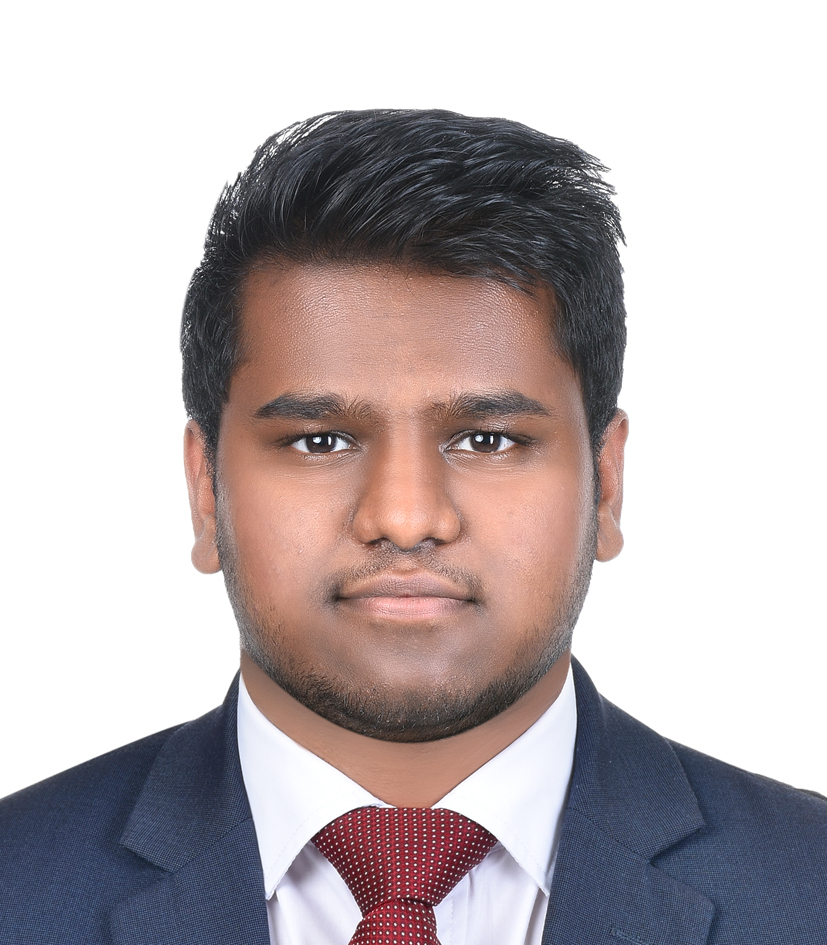
\includegraphics[width=.5\textwidth]{setup/pics/pp2.jpg} % Picture
        \end{minipage} \hfill
        \begin{minipage}{0.95\textwidth} % Name and Contact Info
            \name{JACINTH DANIEL MOSES}{Computer Science Student} % Name and Profession
            \vspace{2em}
            %\address{United Arab Emirates} $\cdot$
            \email{jackdanielmoseshs@gmail.com} $\cdot$ 
            \linkedin{https://www.linkedin.com/in/tealmint/}{TealMint} $\cdot$
            \github{https://github.com/JacDM}{JacDM} $\cdot$\\
            \phone{+971 56 210 0384} $\cdot$
            \website{https://jacdm.github.io/}{Website}
        \end{minipage}
        
    \end{tcolorbox}

    %%% Sections %%%
    \vspace*{-1em}
    \tcbset{colframe=white,colback=white,arc=5mm,}
    \begin{tcolorbox}
        \vspace*{-0.5em}
        \begin{minipage}[t]{0.28\textwidth} % Side Panel (e.g. Skills, Links, Languages, etc.)
            \begin{tcolorbox}[height=.83\textheight, grow to left by=0.6cm,colback=backdrop,colframe=backdrop,arc=2mm]
                \Label{\ColorHighlight}{Location:UAE}
                
\includegraphics[align=c, width=2.3em]{setup/pics/flags/AE.png}
                \Label{\ColorHighlight}{Nationality:Kenyan}
                
\includegraphics[align=c, width=2.3em]{setup/pics/flags/KE.png}
                \Label{\ColorHighlight}{Ethnicity: Indian}
                
\includegraphics[align=c, width=2.3em]{setup/pics/flags/IN.png}
                \Label{\ColorHighlight}{DOB: 26 February 2003}
                % Skills, the skill level is drawn as bars, input: skill name and an array starting from 0 and ending before 4
                \subsection*{Coding Languages}
                    \skills{Java}{0, 1, 2, 3, 4}
                    \skills{Python}{0, 1, 2, 3}
                    \skills{C\#}{0, 1, 2, 3}
                \subsection*{Technical Skills}
                    \skills{Linux/WSL}{0, 1, 2, 3}
                    \skills{Unity}{0, 1, 2, 3}
                    \skills{\LaTeX}{0, 1, 2, 3}
                    \skills{Git}{0, 1, 2, 3}
                    \skills{Docker}{0, 1, 2}
                    $\cdot$ Used latex to make this CV!
            \end{tcolorbox}
        \end{minipage}
        \begin{minipage}[t]{0.75\textwidth} % Main Panel (e.g. Education, Work Experience)
            \begin{tcolorbox}[grow to right by=0.75cm,height=0.8\textheight,colframe=white,colback=white]
                \vspace{-3em}
                % Profile Section
                \section*{Profile}
                %\SimpleSeparator{\ColorTextMain}
                \vspace{-1em} 
                With many years of experience tinkering with hardware such as Raspberry Pi's and Linux machines 
                I have developed a passion for learning about the inner workings of computers. I have also developed a passion for programming 
                and writing code in languages such as Java, Python, etc.
                I enjoy delving deeper into technologies and understanding how they fundamentally work.
                %\SimpleSeparator{\ColorTextMain}
                % Work Experience
                \vspace{-2em}
                \section*{Projects}
                \vspace{-1em}
                    \work{Group Software Development Project}{October 2022 - March 2023}{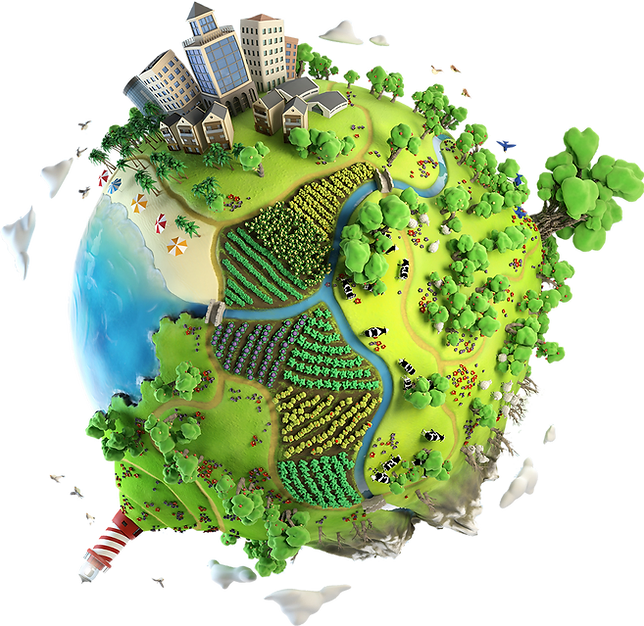
\includegraphics[align=c, width=2em]{setup/pics/globe.png} Year 3@Heriot-Watt}{
                        •GeoTagAR was a 6 - month project developed by me and my team to providing users from all over the world with a way to connect and share AR-based content.\\
                        • My roles included developing the Front and Backend of the application using the ARCore framework for AR and Flutter for the frontend. In addition, I was apointed as the team leader and scrum master. \\ 
                        • \href{https://mintsolutions.wixsite.com/tech}{Company Website}\\
                        • \href{https://github.com/JacDM/GeoTagAR}{Code Repository}

                    }\vspace{1em}

                    \work{Brakeys Game Jam 2020.2}{August 2022}{itch.io}{
                        • This was my first attempt at a game jam, where I built a 2D game called buggy land where you had to Navigate through an extremely glitchy map and try to beat the game.\\
                        • \href{https://jacdanielmoses.itch.io/buggy land}{Game Link}\\
                    }
                \vspace{-3em}
                % Education
                \section*{Education}
                \vspace{-1em}
                    \education{BSc(Hons) Computer Science}{September 2021 - May 2024}{%
\includegraphics[align=c, width=2em]{setup/pics/HW.png} 
                    Heriot-Watt University - Dubai}{
                        \vspace*{0.3em} \noindent \large \color{title} \parbox{.7\linewidth}{\textsl{Year 3, Semester 2}} \par \color{black} \small
                        \Label{}{\href{https://curriculum.hw.ac.uk/coursedetails/F29FB?termcode=202223}{Foundations 2}}
                        \Label{}{\href{https://curriculum.hw.ac.uk/coursedetails/F29PD?termcode=202223}{Professional Development}}
                        \Label{}{\href{https://curriculum.hw.ac.uk/coursedetails/F29OC?termcode=202223}{Operating Systems \& Concurrency}}\\
                        \Label{}{\href{https://curriculum.hw.ac.uk/coursedetails/F29LP?termcode=202223}{Language Processors}}\\
                        \noindent \large \color{title} \parbox{.7\linewidth}{\textsl{Year 3, Semester 1}} \par \color{black} \small
                        \Label{}{\href{https://curriculum.hw.ac.uk/coursedetails/F29AI?termcode=202223}{AI and Intelligent Agents}}
                        \Label{}{\href{https://curriculum.hw.ac.uk/coursedetails/F29DC?termcode=202223}{Data Communications and Networking}}
                        \Label{}{\href{https://curriculum.hw.ac.uk/coursedetails/F29FA?termcode=202223}{Foundations 1}}
                        \Label{}{\href{https://curriculum.hw.ac.uk/coursedetails/F29SO?termcode=202223}{Software Engineering}}
                        %\Label{}{\href{https://curriculum.hw.ac.uk/coursedetails/F28DA?termcode=202223&programmeCode=F291-COS&campuscode=}{Data Structures and Algorithms}}

                        } \vspace{1em}
                    \education{International Advanced Level}{September 2019 - May 2021}{%
\includegraphics[align=c, width=1.5em]{setup/pics/RAK.jpeg} 
                    RAK Academy}{
                        \Label{}{Edexcel Mathematics - A*}
                        \Label{}{CIE Computer Science - A}
                        \Label{}{Edexcel Physics - B}    \\
                        } 

                        \education{IGCSE}{September 2017 - May 2019}{%
\includegraphics[align=c, width=1.5em]{setup/pics/RAK.jpeg}
                         RAK Academy}{
                            \Label{}{Edexcel Mathematics - A*}
                            \Label{}{CIE Computer Science - A}
                            \Label{}{CIE Additional Maths - B}\\
                            \Label{}{CIE First Language English-B}
                            \Label{}{CIE Physics-B}
                            \Label{}{CIE Literature-B}\\
                            \Label{}{Edexcel Psychology}
                            \Label{}{CIE Business Studies}
                            \Label{}{CIE Design Technology}
                            }

                

            \end{tcolorbox}
        \end{minipage}

    \end{tcolorbox}
    \newpage % Start a new page

    \vspace*{-1em}
    \tcbset{colframe=white,colback=white,arc=5mm,}
    \begin{tcolorbox}
        \vspace*{-0.5em}
        \begin{minipage}[t]{0.28\textwidth} % Side Panel (e.g. Skills, Links, Languages, etc.)
            \begin{tcolorbox}[height=\textheight, grow to left by=0.6cm,colback=backdrop,colframe=backdrop,arc=2mm]
                \subsection*{Languages}
                \Label{\ColorHighlight}{English} \\
                $\cdot$ LSRW 
                $\cdot$ Fully Proficient\\

                \Label{\ColorHighlight}{Tamil}\\
                $\cdot$ LS 
                $\cdot$ Native Language\\

                \Label{\ColorHighlight}{Hindi}\\
                $\cdot$ LS 
                $\cdot$ Conversational
            \end{tcolorbox}
        \end{minipage}
        \begin{minipage}[t]{0.75\textwidth} % Main Panel (e.g. Education, Work Experience)
            \begin{tcolorbox}[grow to right by=0.75cm,height=\textheight,colframe=white,colback=white]

                % Awards
                \section*{Awards}
                    \education{Undergraduate Merit Scholarship}{2021}{Heriot-Watt University - Dubai}{
                        A 50\% scholarship for my undergraduate degree based on A-Level results.\\
                    } \vspace{1em}
                    \education{Best Sungura Scout}{2011}{Oshwal Academy Nairobi Primary}{
                        A rotating shield given to me in primary on the basis of my performance on a 3-day field trip\\
                    } \vspace{1em}
                \vspace{-2em}

                % Certifications
                \section*{Certifications}
                    \education{Data Science R Basics}{June 2022}{DataCamp}{
                        Learning how to use R for basic data science tasks.\\
                        \href{https://www.datacamp.com/statement-of-accomplishment/course/8255e858f885b3d4389a21bec2d3c4e29b36315c}{Link}\\
                    } \vspace{1em}
                \vspace{-2em}

                % Volunteering
                \section*{Volunteering}
                    \work{Deputy Head Boy}{October 2019 - July 2020}{RAK Academy}{
                        • My responsibilities included setting up events, being the student voice, commissioning varsity jackets for my graduating class etc.\\
                    }
                    \vspace{1em}
                    \work{Altar Server}{February 2018 – Jan 2022}{St. Lukes RAK}{
                        •	My responsibilities varied from week to week from being the thurifer to cross-bearing and helping the priest with the preparation of the table for communion.\\
                    }
                    \vspace{1em}
                    \work{Windows Insider}{February 2020 - Present}{Microsoft}{
                        •	My responsibilities include testing new versions of windows and providing 
                        feedback by identifying bugs and submitting tickets for them.\\
                    }
                \vspace{-2em}
                \section*{Extra Curricular}
                    \education{Interests/Hobbies}{}{}{
                        \Label{}{Docker}
                        \Label{}{Linux}
                        \Label{}{Operating systems (Windows Insider)}\\
                        \Label{}{Beta testing for various applications}
                        \Label{}{Game Development (Unity)}\\
                        \Label{}{Running a Minecraft server/Gaming}\\
                    } \vspace{1em}

            \end{tcolorbox}
        \end{minipage}
    \end{tcolorbox}
\end{document}
